\section{Project Data}

\begin{table}[h!]
    \begin{tabular}{l|l|l}
        \textbf{Item}            & \textbf{URL}                              & \textbf{Revision}\\\hline
        Source Code Experimental & \url{https://github.com/martinnj/PCDS}    & \texttt{8a592e1}\\
        % https://github.com/martinnj/PCDS/commit/8a592e18000385fd05c455068b48f9e940a16944
        Source Code Production   & \url{https://github.com/martinnj/Leapkit} & \texttt{7c6ffbc}\\
        % https://github.com/martinnj/Leapkit/commit/7c6ffbc096699d20c9bfeabbcfa2db91f0d2b204
        Scrum board              & \url{https://trello.com/b/lF49jIHe}       & \texttt{N/A}
    \end{tabular}
    \label{tab:projdata}
    \caption{For access to the board/repositories, please contact any group member.}
\end{table}

\begin{figure}
  \begin{center}
   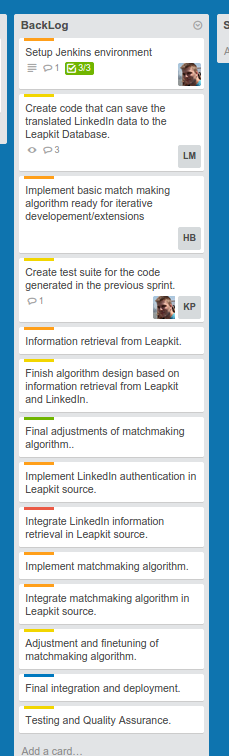
\includegraphics[width=0.3\textwidth]{backlog.png}
   \caption{The project backlog as seen in Trello.}
   \label{fig:backlog}
 \end{center}
\end{figure}

Our project backlog can be seen in figure \ref{fig:backlog}


